\documentclass[dvipdfmx,uplatex]{jsarticle}
\title{情報リテラシー(演習)第2回}
\author{
    名前: 長田悠生\\
    学籍番号: 202310330
}
\date{2023/6/5}

\usepackage[dvipdfmx]{graphicx}

\begin{document}
  \begin{titlepage}
    \maketitle
    \begin{center}
      \textmc{\HUGE \LaTeX}
    \end{center}
    \thispagestyle{empty}
  \end{titlepage}

  \centerline{\LARGE 選んだ分野・領域: 情報学・計算機・ソフトウェア}
  \vspace{10mm}
  \textmc{\LARGE 概要\\}
  \textmc{
    ソフトウェア分野は、単なるソフトウェア開発にとどまらず、大規模計算やアルゴリズム、プログラミング言語の開発など多岐にわたる分野である。
    ソフトウェア分野で多種多様な研究が行われている所以は、ソフトウェアの性能向上のため(アルゴリズムの研究などが挙げられるだろう。)である部分が大きい。
    また、インターネットの普及に伴って、ウェブアプリケーションの利用者が増加し、サーバー負荷の分散をどのように行うか等の研究を行う必要も出てきた。
    近年注目されているAIやIoTなどによって、ますますソフトウェアの需要が高まっているだろう。\\
    \quad ソフトウェアの研究分野は、時代の変化とともに研究分野が目まぐるしく変化するそんなダイナミックな研究分野なのである。\\
  }
  \begin{figure}[h]
    \begin{center}
      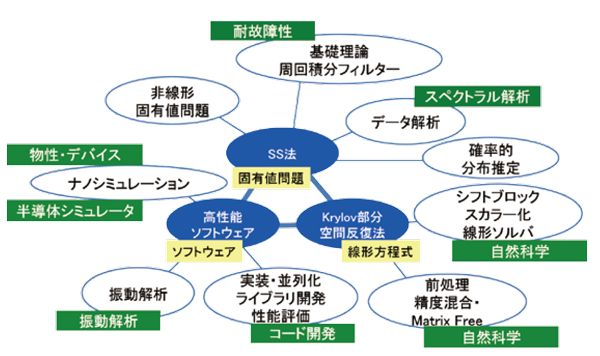
\includegraphics[width=100mm]{31sakurai02.png}
      \caption{アルゴリズムとソフトウェアの関係}
    \end{center}
  \end{figure}
  \\[10pt]
  \textmc{\LARGE 理由\\}
  \textmc{
    私は、高校時代から統計解析とウェブアプリケーション開発を行ってきました。
    そのため、ソフトウェア分野には昔から強い興味がありました。ソフトウェア分野に興味を持ち始めた理由は、
    自分で組んだ統計解析のプログラムを多くの人に使ってもらうためにウェブアプリケーションを作成したのが始まりでした。
    それから、ブログアプリケーションや生徒管理システムを作成する中で、サーバーの負荷分散やセキュリティ関係にも興味を持つようになりました。
    ソフトウェア分野は、変化がちとても激しく、1年後にはもはや別世界になっているような世界です。
    私は、この分野の変化がとても激しいことで一度も飽きることなくソフトウェア開発に従事してきました。そして、これからもこの分野を自由気ままに楽しんでいこうと思います。
  }
  \\[10pt]
  \begin{thebibliography}{99}
    \item 図1の引用元: "技術革新を支えるアルゴリズムと ソフトウェアを開発 先端数値解析ソフトウェアリサーチユニット", https://ura.sec.tsukuba.ac.jp/archives/6580
  \end{thebibliography}


\end{document}
